\section{Anwendung}

\subsection{Datenkompression}

\subsubsection{Notation}
\begin{tabular}{ll}
$f$ & diskretes Signal\\
$B$ & Bit-Stream, repräsentiert eine Approximation von $f$ welches mit einer bestimmten Methode codiert wurde. \\
$\tilde{f}$ & Approximation von $f$ repräsentiert durch B, die komprimierte Version von $f$\\
$r$ & Kompressionsrate (zB.: $\dfrac{\text{Anzahl Bits in }f}{\text{Anzahl Bits in }B}$)\\
$\tilde{f}-f$ & Quantisierungsfehler, Quantisierungsrauschen, Verzerrung, Residual\\
\end{tabular}
\begin{tabular}{ll}
$\mathrm{MSE}(\tilde{f}) := \frac{1}{M \cdot N}\sum_{i=0}^{M-1}\sum_{k=0}^{N-1}\lvert \tilde{f}_{i,k}-f_{i,k} \rvert^2$ & Mean Squared Error vom komprimierten Bild\\
$\mathrm{PSNR}(\tilde{f}) := 10 \cdot \log_{10}(\frac{K^2}{\mathrm{MSE}(\tilde{f})})$ & Peak Signal to Noise Ratio, mit $K=\mathrm{max}\{\mathrm{max}(f)-\mathrm{min}(f)\}$ \\
 &  (Bei eine Graustufenbild mit der Farbtiefe 8 beträgt $K=255$)
\end{tabular}

\subsubsection{Vorgen für Datenkompression}
\[ 
	f \longrightarrow \boxed{\mathrm{Transformation}} \longrightarrow (c_k)_{k\in J} \longrightarrow \boxed{\mathrm{Quantisierung}} \longrightarrow (\tilde{c}_k)_{k \in J} \longrightarrow \boxed{\mathrm{Entroipy Coding}}\longrightarrow B 
\]

Ziel ist es das Signal $f$ in eine Basis zu Transformieren, bei der viel Koeffizienten 0 oder sehr klein werden. Bei der Quantisierung werden diese kleinen Koeffizienten auf 0 quantisiert. Diese Koeffizienten können durch eine effizientes Entropy Coding komprimiert abgespeichert werden.\\

Waveletkompression:
\begin{itemize}
	\item Analyse Wavelet: sollte einige verschwindende Momente haben
	\item Synthese Wavelet: die synthese Funktion sollte eine gute Regularität aufweisen
	\item alle Funktionen sollten Symmetrisch sein (gerade oder ungerade, "Lineare Phase")
	\item Orthogonalität
	\item kurze Filter für bessere Performance (Mehr verschwindende Momente und bessere Regularität erhöhen die Filterlänge)
\end{itemize}
Ein gutes Wavelet ist das bior4.4. Es ist biorthogonal, symmetrisch, hat 4 vanishing Moments, das Synthese Wavelet hat eine Regularität die grosser als 1.3 ist. Die resultierenden Filter weisen 7 bzw. 9 Filterkoeffizienten auf.

\subsubsection{Zwei-Dimensionale Wavelettransformation}

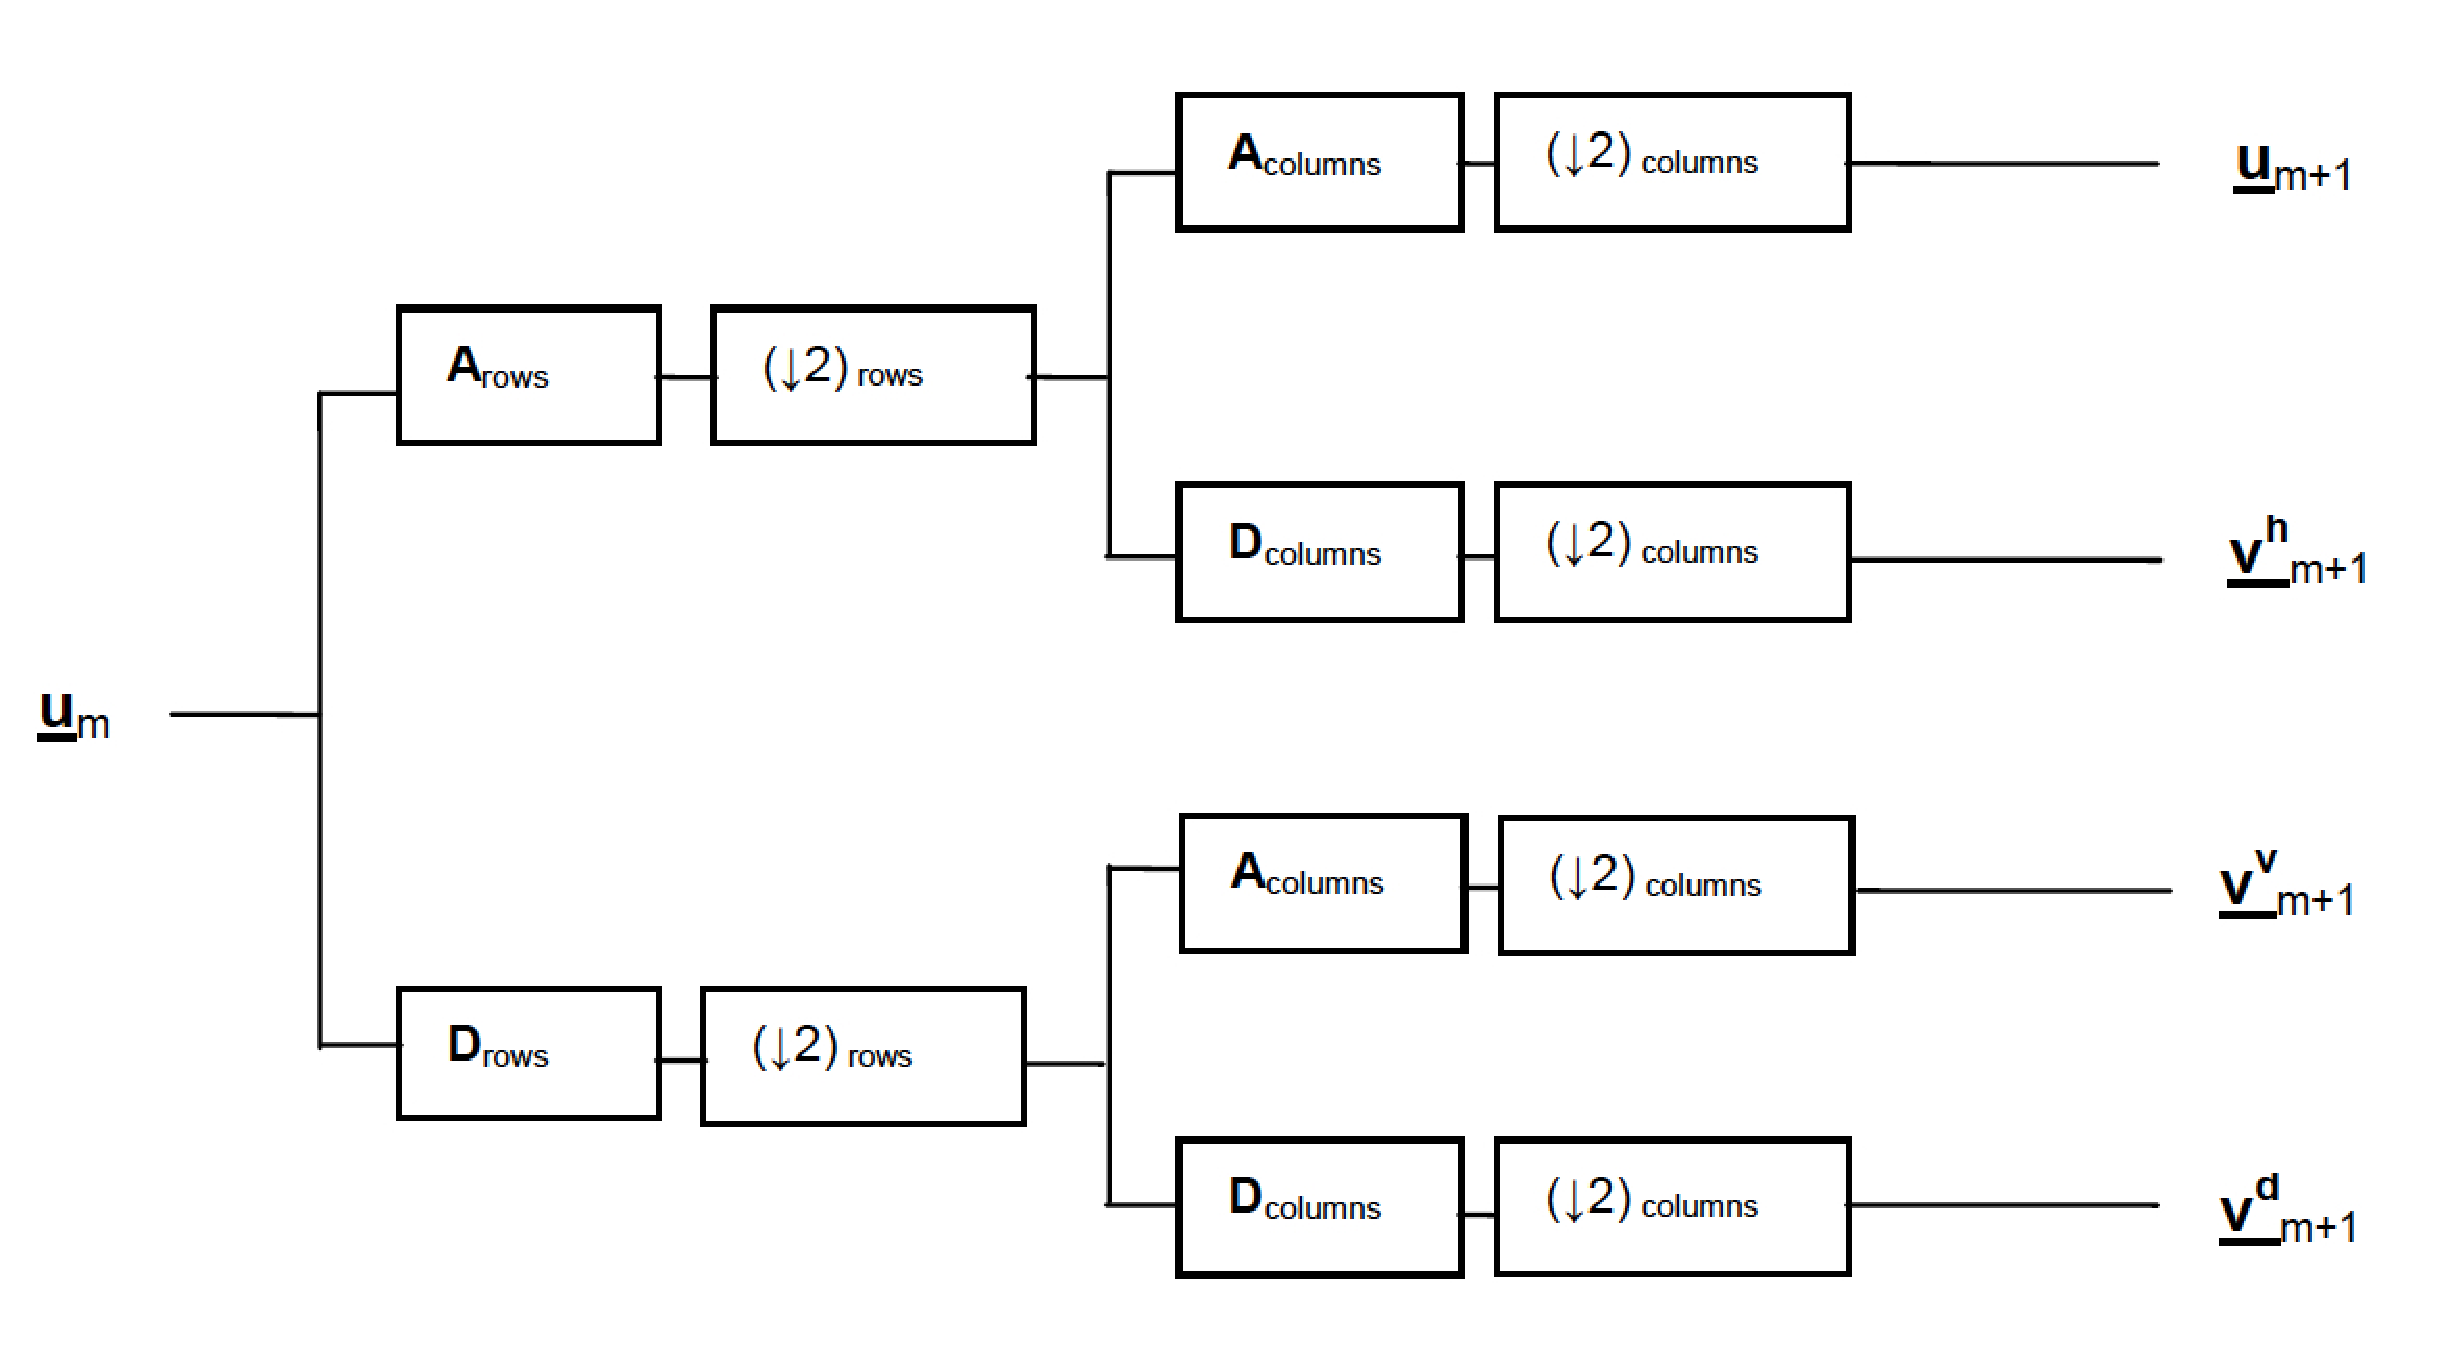
\includegraphics[width=\textwidth]{content/ZweiDimWaveletTransf.pdf}

%TODO MRA Formeln



\subsection{Denoising}

\subsection{Feature Detection and Extraction}

\subsection{Matlab}